%%%%%%%%%%%%%%%%%%%%%%%%%%%%%%%%%%%%%%%%%%%%%%%%%%%%%%%%%%%%%%%
%
% Welcome to Overleaf --- just edit your LaTeX on the left,
% and we'll compile it for you on the right. If you open the
% 'Share' menu, you can invite other users to edit at the same
% time. See www.overleaf.com/learn for more info. Enjoy!
%
%%%%%%%%%%%%%%%%%%%%%%%%%%%%%%%%%%%%%%%%%%%%%%%%%%%%%%%%%%%%%%%
\documentclass[unicode,11pt]{beamer}
\usepackage[whole,autotilde]{bxcjkjatype}
\usepackage{minted}
\usetheme{Madrid}
\definecolor{links}{HTML}{2A1B81}
\hypersetup{colorlinks,linkcolor=,urlcolor=links}

\title{システム情報工学特論}
\subtitle{コードで学ぶAWS入門 - 第一回}
\author{真野智之 (Tomoyuki Mano)}
\institute[OIST]{Okinawa Institute of Science and Technology}
\date{2022/06/08 @東大工学部}

\begin{document}

\frame{\titlepage}

\begin{frame}{自己紹介}
真野智之 (Tomoyuki Mano)
\begin{itemize}
    \item 東京大学情報理工学系研究科システム情報学専攻博士課程修了 (2021年)
    \item 現職: 日本学術振興会特別研究員(PD),沖縄科学技術大学院大学フェロー
    \item 大学院時の研究: マウスの脳の三次元画像解析,クラウドを使ったデータベース構築
    \item 現在の研究: 頭足類(タコ・イカ) の脳の研究: 擬態(camouflage) を生み出す脳の神経回路を生成モデルの視点で解析しようとしている
    (
    \href{https://twitter.com/CephWarden/status/1142083856893263872}{1},
    \href{https://twitter.com/CephWarden/status/1384644335069667334}{2},
    \href{https://twitter.com/CephWarden/status/1232307456346181632}{3}
    )
    \item 講義に関する質問などは次の連絡先まで. tomoyukimano@gmail.com
\end{itemize}
\end{frame}

\begin{frame}{成績評価}
\begin{itemize}
    \item 成績は期末レポート (課題内容は後日発表) で評価します
\end{itemize}
\end{frame}

\begin{frame}{講義について (1)}
\begin{itemize}
    \item 講義資料は
    \url{https://tomomano.github.io/learn-aws-by-coding/}\\
    にあります.
    \item ハンズオンで使用するソースコードは \url{https://github.com/tomomano/learn-aws-by-coding}\\
    にあります
    \item スライドと課題のアナウンスは
    \url{https://github.com/tomomano/intro-aws-2022}\\
    にあります
\end{itemize}
\end{frame}

\begin{frame}{講義について (2)}
\begin{itemize}
    \item 講義の中盤 (40分前後) で一度休憩をとります.
    この際に質問などにも答えます.
    \item 講義に関する質問は Zoom のチャットに飛ばして下さい.
    できるだけすぐにその場で回答します.
    \item 講義の内容は
    \url{https://tomomano.github.io/learn-aws-by-coding/}\\
    に従って行います.
    講義ではコードのデモなど行いますが,基本的に伝える情報は資料と同じです.
    余裕のある人は各自のペースでどんどん先に進んでしまって構いません.
    \item ハンズオンのプログラムでバグなど発見した場合は
    \href{https://github.com/tomomano/learn-aws-by-coding/issues}{GitHub の Issues}
    まで報告してもらえると助かります (残念ながら成績には関係ありません).
\end{itemize}

\end{frame}

\begin{frame}{書籍紹介}

\begin{columns}
    \begin{column}{0.47\textwidth}
        \begin{itemize}
            \item 2020年,2022年に行った講義資料がネットでバズり,2021年9月にマイナビ出版さんから出版されました.
            \item 講義資料は引き続きウェブで無料公開しています.
        \end{itemize}
    \end{column}
    \begin{column}{0.5\textwidth}
        \begin{figure}
            \centering
            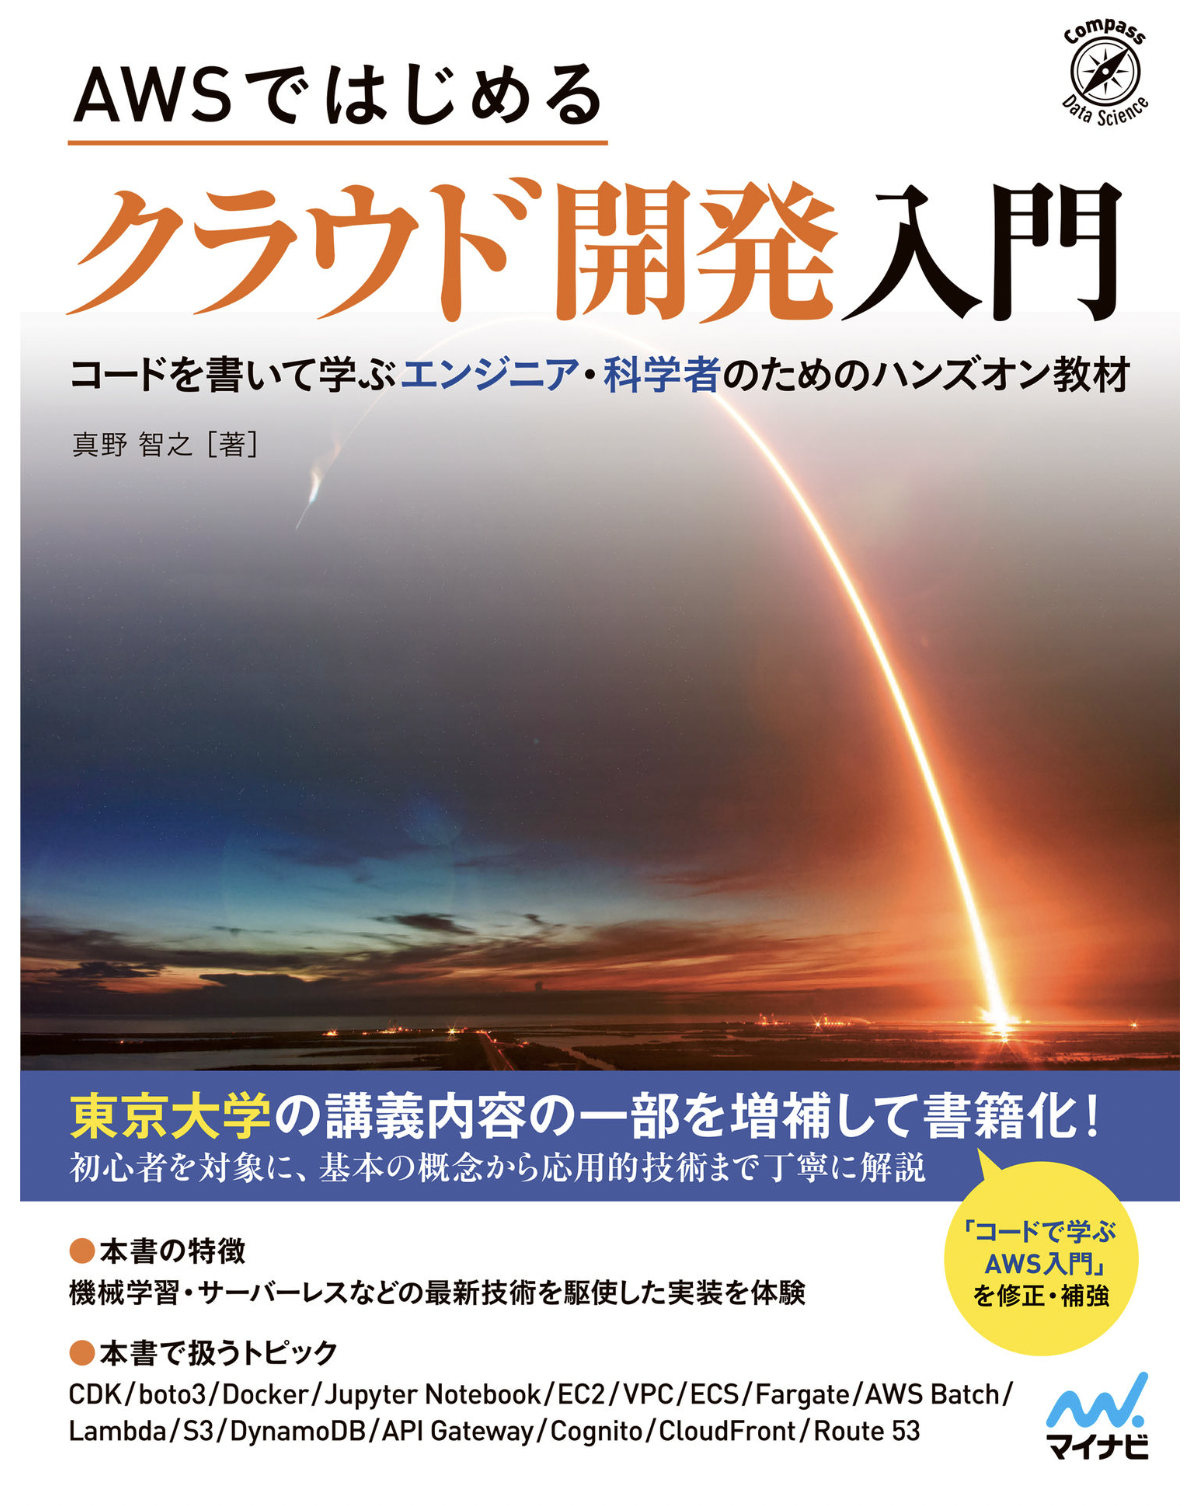
\includegraphics[width=0.8\textwidth]{cover.png}
        \end{figure}
    \end{column}
\end{columns}

\end{frame}

\begin{frame}{講義の予定}
    \begin{itemize}
        \item 第一回 (6/08): イントロダクション・セットアップ
        \item 第二回 (6/15): EC2 入門
        \item 第三回 (6/22): クラウドを使った深層学習入門
    \end{itemize}
\end{frame}

\begin{frame}{環境のセットアップ (1)}

\href{https://tomomano.github.io/learn-aws-by-coding/#sec:appendix_settingup}{講義資料 "15. Appendix: 環境構築"} を参照のうえ,自身の計算機で
以下の環境を構築せよ.

\begin{itemize}
    \item Python のインストール
    \item Node.js のインストール
    \item AWS CLI のインストール
    \item AWS CDK のインストール
\end{itemize}

Mac/Linux ユーザーは OS に標準搭載のシェルを使用すればよい.
Windows ユーザーは, \href{https://docs.microsoft.com/en-us/windows/wsl/install}{WSL} により仮想 Linux 環境を構築することを推奨する.

\end{frame}

\begin{frame}[fragile]
\frametitle{環境のセットアップ (1) -- 確認}

前スライドでの準備が正しく完了しているか,以下のコマンドをシェルで実行せよ.
ソフトのバージョンが表示されればOK.

\rule{\textwidth}{1pt}

\begin{semiverbatim}
python --version
node --version
aws --version
cdk --version
\end{semiverbatim}

\rule{\textwidth}{1pt}

\end{frame}

\begin{frame}[fragile]
\frametitle{講義専用アカウントの使い方 (1)}

\begin{itemize}
    \item 真野から各学生のメールアドレスにログイン情報を記述したテキストファイル (JSON ファイル) が送信されます.
    \item 適当なテキストエディターでこれを開くと以下のような内容が書いてあるはずです.
    \begin{semiverbatim}
    \{
        "UserName": "student-XXX",
        "Password": "ABCDEF",
        "AccessKeyId": "XXXXXXXXX",
        "SecretAccessKey": "YYYYYYYY",
        "Sign in link": "https://ZZZZZZZ"
    \}
    \end{semiverbatim}
    \item このログイン情報は決して漏洩することのないよう注意して管理すること.
\end{itemize}
    
\end{frame}

\begin{frame}{講義専用アカウントの使い方 (2)}

\begin{itemize}
    \item AWSコンソールにログインするには, "Sign in link" にアクセスし, "UserName" と "Password" を入力してください.
    \item AWS CLI / CDK を使うには,"AccessKeyId", "SecretAccessKey" を使用してください.
\end{itemize}
    
\end{frame}

\begin{frame}{講義専用アカウントの注意点}

\begin{itemize}
    \item このアカウントは今日の講義の時間中のみ有効です.
    講義が終わったあとは,数時間以内に削除されることに注意してください.
    \item この講義のために \$500 のクレジットが付与されています.
    この \$500 を受講者全員で共有している状態です.
    (ないとは思いますが) 大量の計算を走らせるとこのクレジットが枯渇してしまいますので,講義のハンズオン以外の目的には使用しないようにしてください.
\end{itemize}

\end{frame}

\end{document}

